% ChurnMaster two-page report (conference style; colour figure, black-and-white text).
% Build:  python report/make_figure.py   (regenerates fig_results.pdf from results/eval/summary.csv)
%         python report/verify_report.py (cross-checks every number against results/, configs/, src/)
%         pdflatex churnmaster_report.tex  (run twice for cross-references)
\documentclass[9pt,twocolumn]{extarticle}
\usepackage[letterpaper,left=0.6in,right=0.6in,top=0.55in,bottom=0.6in,columnsep=0.22in]{geometry}
\usepackage[T1]{fontenc}
\usepackage{newtxtext,newtxmath}
\usepackage[protrusion=true,expansion=true]{microtype}
\usepackage{graphicx,booktabs,amsmath,array,multirow}
\usepackage[hidelinks]{hyperref}
\usepackage[font=footnotesize,labelfont=bf,labelsep=period,skip=3pt]{caption}
\usepackage{enumitem}
\setlist[itemize]{nosep,leftmargin=1.1em,labelsep=0.45em}
\usepackage{titlesec}

% ---- Heading hierarchy (black only) -------------------------------------------
% Level 1: numbered, bold, title case.  Level 2: numbered, italic.  Inline
% labels inside paragraphs: bold run-in text ending in a period (\inl).
\titleformat{\section}{\normalsize\bfseries}{\thesection}{0.6em}{}
\titlespacing*{\section}{0pt}{5pt plus 1pt minus 1pt}{2pt plus 1pt}
\titleformat{\subsection}{\normalsize\itshape}{\thesubsection}{0.5em}{}
\titlespacing*{\subsection}{0pt}{3pt plus 1pt minus 1pt}{1pt plus 0.5pt}
\newcommand{\inl}[1]{\mbox{\textbf{#1.}}\ }

\setlength{\parindent}{1em}
\setlength{\parskip}{0pt}
\renewcommand{\topfraction}{0.9}\renewcommand{\dbltopfraction}{0.9}\renewcommand{\textfraction}{0.08}\renewcommand{\floatpagefraction}{0.85}\setcounter{topnumber}{3}\setcounter{totalnumber}{4}
\setlength{\textfloatsep}{8pt plus 2pt minus 2pt}
\setlength{\floatsep}{6pt plus 2pt minus 2pt}
\setlength{\dbltextfloatsep}{8pt plus 2pt minus 2pt}
\setlength{\abovecaptionskip}{3pt}
\AtBeginDocument{%
  \setlength{\abovedisplayskip}{4pt plus 1pt minus 1pt}%
  \setlength{\belowdisplayskip}{4pt plus 1pt minus 1pt}%
  \setlength{\abovedisplayshortskip}{2pt plus 1pt}%
  \setlength{\belowdisplayshortskip}{3pt plus 1pt minus 1pt}}
\clubpenalty=10000 \widowpenalty=10000 \displaywidowpenalty=10000
\pagestyle{plain}
\raggedbottom

\newcommand{\act}[1]{\textsc{#1}}
\newcommand{\pol}[1]{\textit{#1}}
\newcommand{\Lset}{\mathcal{L}}

\begin{document}

\twocolumn[{%
\begin{center}
{\LARGE\bfseries ChurnMaster: Learning Routing-Table Maintenance\\[2pt]
for a Kademlia-like DHT under Churn with Tabular Q-Learning\par}
\vspace{6pt}
{\normalsize Deepansh Singh \qquad Ankur Kumar\par}
\vspace{3pt}
{\small AI2 Course Mini-Project \quad$\cdot$\quad Code: \url{https://github.com/Ankurkumar359/ChurnMaster} \quad$\cdot$\quad Release tag: \texttt{v1.2.0}\par}
\end{center}
\vspace{0pt}
}]

\section{Introduction}
In a Kademlia DHT~\cite{kad}, each node keeps up to $k$ contacts per XOR-distance bucket. Under churn, contacts go offline, and the node must decide when to ping a contact and when to replace it with a cached candidate. Pinging costs messages, whereas dead entries cause lookup timeouts. Standard Kademlia pings the least-recently-seen contact whenever a newcomer is offered to a full bucket; this rule is robust but message-heavy.

\inl{Objective} We ask whether a tabular Q-learning policy~\cite{wat,sb} that uses only locally observable signals can trade maintenance traffic against lookup success and latency better than (a)~Kademlia-style maintenance, (b)~a random policy with the same action frequencies, and (c)~a tuned rule-based heuristic, and whether it transfers to an unseen churn level. Hypotheses H1--H5 were pre-registered and are reported whether or not they pass.

\section{RL Formulation}
\subsection{Environment}
The environment is a deterministic, pure-Python discrete-event simulator of a 128-node DHT with 8-bit identifiers, which gives the focal node $F$ eight buckets. Each bucket holds $k=4$ contacts and a four-entry replacement cache (TTL 300\,s); lookups use parallelism $\alpha_{\mathrm{L}}=2$ and are served by the 3 closest online replicas. Round-trip times are log-normal and packets are lost with probability 0.02. Only $F$ adapts; all other nodes rebuild stale routing tables every 300\,s. Lookups arrive at 1/s with uniform keys and run atomically with a 2000\,ms deadline. An episode consists of 600\,s of warm-up and 2400\,s of measurement, with one decision epoch every 30\,s. Each node alternates Weibull-distributed sessions (shape 0.6) with exponential downtimes. Policy-independent randomness (loss, jitter, table rebuilds) is keyed by event identity, so different policies observe identical outcomes for identical messages.

\subsection{State Representation}
\inl{Agent observations} At every epoch, $F$ makes one decision per non-empty bucket. A decision concerns that bucket's least-recently-seen \emph{incumbent} contact and its freshest cached \emph{candidate}, if any.

\inl{Observable features} The agent observes seven features of this pair, each discretized into two or three bins (Table~\ref{tab:state}); a value exactly on a threshold falls into the higher bin. SRTT is the incumbent's smoothed round-trip time.

\par\smallskip\noindent\begin{minipage}{\columnwidth}
\centering\footnotesize
\captionof{table}{The seven discretized state features.}
\label{tab:state}
\setlength{\tabcolsep}{3pt}
\renewcommand{\arraystretch}{1.05}
\begin{tabular}{@{}>{\raggedright\arraybackslash}p{1.45cm} >{\raggedright\arraybackslash}p{2.95cm} >{\raggedright\arraybackslash}p{3.9cm}@{}}
\toprule
Feature (bins) & Categories or thresholds & Meaning\\
\midrule
Tier (3) & top, second, other & Bucket $b=7$, $b=6$, or $b\le5$\\
Failures (3) & $0$, $1$, $\ge 2$ & Consecutive failed pings to incumbent\\
Last reply (2) & $<60$\,s, $\ge 60$\,s & Time since incumbent last replied\\
Age (3) & $<120$, $120$--$1200$, $\ge 1200$\,s & Incumbent's time in the table\\
Candidate (3) & none, fresh ($<30$\,s), stale & Freshest cached; stale is 30--300\,s\\
Faster (2) & yes, no & Cand.\ RTT $<0.7\times$ incumbent SRTT\\
Churn (2) & $<0.10$, $\ge 0.10$ & $F$'s timeout share, last 120\,s\\
\bottomrule
\end{tabular}
\end{minipage}\par\smallskip

\begin{table*}[t]
\centering\small
\caption{Primary evaluation: means over 20 evaluation seeds (RL is the mean of 3 training runs). Higher $J$ and lookup success (succ., \%) are better; lower p95 latency (ms, all lookups) and pings per hour are better. Bold: best of the four policies per $J$, p95 and pings column. $\Delta J$ is RL minus comparator with a 95\% bootstrap CI; all nine differences are significant after Holm correction. Source: \texttt{results/eval/}.}
\label{tab:main}
\setlength{\tabcolsep}{3.6pt}
\begin{tabular}{@{}l *{3}{r r r r}@{}}
\toprule
 & \multicolumn{4}{c}{stable} & \multicolumn{4}{c}{high\_churn} & \multicolumn{4}{c}{heldout\_medium}\\
\cmidrule(lr){2-5}\cmidrule(lr){6-9}\cmidrule(l){10-13}
Policy & $J$ & succ.\,\% & p95 & pings/h & $J$ & succ.\,\% & p95 & pings/h & $J$ & succ.\,\% & p95 & pings/h\\
\midrule
Kademlia-epoch  & 0.9642 & 100.00 & 371 & 383.9 & 0.9619 & 99.66 & 541 & 338.0 & 0.9640 & 99.96 & 466 & 368.7\\
Matched random  & 0.9589 & 99.54 & 644 & 8.0 & 0.9578 & 99.69 & 730 & 48.3 & 0.9603 & 99.43 & 644 & 26.1\\
Tuned heuristic & \textbf{0.9760} & 100.00 & \textbf{371} & 9.3 & \textbf{0.9735} & 99.84 & \textbf{468} & \textbf{38.5} & \textbf{0.9749} & 99.96 & \textbf{379} & \textbf{20.4}\\
Q-learning (RL) & 0.9739 & 100.00 & 457 & \textbf{7.1} & 0.9705 & 99.79 & 554 & 43.8 & 0.9729 & 99.96 & 521 & 22.6\\
\midrule
$\Delta J$, RL $-$ Kademlia-epoch & \multicolumn{4}{c}{$+0.0097$ [$+0.0091$, $+0.0102$]} & \multicolumn{4}{c}{$+0.0085$ [$+0.0065$, $+0.0110$]} & \multicolumn{4}{c}{$+0.0089$ [$+0.0081$, $+0.0098$]}\\
$\Delta J$, RL $-$ Tuned heuristic & \multicolumn{4}{c}{$-0.0021$ [$-0.0030$, $-0.0013$]} & \multicolumn{4}{c}{$-0.0030$ [$-0.0044$, $-0.0017$]} & \multicolumn{4}{c}{$-0.0020$ [$-0.0027$, $-0.0013$]}\\
$\Delta J$, RL $-$ Matched random & \multicolumn{4}{c}{$+0.0149$ [$+0.0061$, $+0.0295$]} & \multicolumn{4}{c}{$+0.0127$ [$+0.0100$, $+0.0160$]} & \multicolumn{4}{c}{$+0.0126$ [$+0.0053$, $+0.0235$]}\\
RL ping change vs.\ Kademlia-epoch & \multicolumn{4}{c}{$-98.1\%$} & \multicolumn{4}{c}{$-87.0\%$} & \multicolumn{4}{c}{$-93.9\%$}\\
\bottomrule
\end{tabular}
\end{table*}

\inl{State-space size} The state index is the mixed-radix combination of the bins,
\begin{equation}
|\mathcal{S}| = 3 \times 3 \times 2 \times 3 \times 3 \times 2 \times 2 = 648 .
\label{eq:states}
\end{equation}
Only 540 of these indices are reachable, because ``candidate faster'' can be \emph{yes} only when a candidate exists, so the 108 combinations of ``no candidate'' with ``faster'' never occur.

\inl{Partial observability} The full network state, including which nodes are online, their types, congestion and other nodes' tables, is hidden from $F$. The agent therefore acts on local bookkeeping only. Treating the discretized observation as a Markov state is an approximation to a partially observable problem~\cite{kaelbling}, so the convergence guarantees of Q-learning do not apply and all claims below are empirical.

\subsection{Actions}
For each decision the agent chooses one of three actions. \act{Keep} sends no message. \act{Probe} pings the incumbent; if the ping fails, the incumbent is evicted and the candidate is tried. \act{Replace} pings the candidate and swaps it in if it answers; it is masked when no candidate exists. Empty slots are filled from the cache at no cost.

\subsection{Reward and Score}
For a measured lookup $i$ with success indicator $S_i\in\{0,1\}$, latency $L_i$ (failed lookups count at their give-up time) and deadline $D=2000$\,ms, the per-lookup loss is
\begin{equation}
\ell_i = (1 - S_i) + w_L \min\!\left(\frac{L_i}{D},\, 1\right).
\label{eq:loss}
\end{equation}
Let $\Lset_{b,k}$ be the lookups whose key falls in bucket $b$ during epoch $k$, and let $P_{b,k}$ and $E_{b,k}$ be the pings and evictions caused by the decision for $(b,k)$. The reward of that decision is
\begin{equation}
r_{b,k} = -\sum_{i\in\Lset_{b,k}} \ell_i \;-\; \bigl(w_M P_{b,k} + w_R E_{b,k}\bigr),
\label{eq:reward}
\end{equation}
with weights $w_L=0.3$, $w_M=0.1$ and $w_R=0.15$. Over an episode with $N$ measured lookups, $P$ pings and $E$ evictions, the evaluation score is
\begin{equation}
J = 1 - \bar{\ell} - \frac{w_M P + w_R E}{N} = 1 + \frac{1}{N}\sum_{b,k} r_{b,k},
\label{eq:score}
\end{equation}
where $\bar{\ell}$ is the mean of~\eqref{eq:loss}. The identity in~\eqref{eq:score} held on every diagnosed episode (maximum error $3.3\times10^{-16}$).

\subsection{Tabular Q-Learning}
The action-value function $Q$ is a $648\times3$ table initialised to zero. Each one-epoch bucket transition $(s,a,r,s')$, with $s'$ the same bucket's state at the next epoch, triggers the update
\begin{equation}
Q(s,a) \leftarrow Q(s,a) + \alpha_n \Bigl[\, r + \gamma \max_{a'\in\mathcal{A}(s')} Q(s',a') - Q(s,a) \Bigr],
\label{eq:qupdate}
\end{equation}
where $\mathcal{A}(s')$ is the set of allowed actions in $s'$, $\gamma$ is the discount factor, and the step size $\alpha_n=\max\bigl(\alpha_{\min},(1+n)^{-0.7}\bigr)$ depends on the number $n$ of earlier updates of $(s,a)$. Transitions that span an empty bucket or the episode end are dropped. Exploration is $\epsilon$-greedy, with $\epsilon$ decaying linearly from 1.0 to 0.05 over the first 60\% of episodes; greedy ties break in the order \act{Keep}, \act{Probe}, \act{Replace}. A grid search on validation seeds selected $\gamma=0.8$ and $\alpha_{\min}=0.02$.

\section{Experimental Setup}
\inl{Scenarios} Nodes are either stable or flaky. \pol{stable} has 70\% stable nodes, mean sessions of 4\,h (stable) and 30\,min (flaky), and 20\,min downtimes; \pol{high\_churn} has 30\%, 1\,h/5\,min sessions and 10\,min downtimes; \pol{heldout\_medium} has 45\%, 2\,h/10\,min sessions and 12\,min downtimes. The last scenario is never used for training or tuning.

\inl{Training} We train 3 independent runs of 200 episodes each, alternating stable and high\_churn episodes, and validate every 20 episodes on 5 separate seeds per training scenario.

\inl{Baselines} \pol{kademlia\_epoch} probes whenever a candidate exists, applied at the shared 30\,s decision points. \pol{matched\_random} samples actions with RL's own frequencies, which tests whether \emph{where} RL acts matters. \pol{tuned\_heuristic} is the best of 32 rule configurations on training seeds; RL's table can represent every configuration exactly. The evaluation also includes \pol{never\_replace}, \pol{always\_replace}, \pol{uniform\_random}, real-protocol \pol{kademlia\_std}, the default heuristic, a privileged per-scenario heuristic and a ground-truth \pol{oracle} (a reference, not an upper bound).

\inl{Evaluation protocol} The 20 evaluation seeds per scenario were locked before evaluation and checked against 635 other seed states for overlap (none). The evaluation ran once: 780 episodes ($13$ policy labels $\times$ 3 scenarios $\times$ 20 seeds), where the 13 labels are the 10 baselines above plus the 3 independently trained RL runs. RL denotes the per-seed mean of these 3 runs. Comparisons are paired by seed, with 95\% percentile-bootstrap confidence intervals (10\,000 resamples) and Wilcoxon signed-rank tests. The 9 primary tests (RL versus \pol{kademlia\_epoch}, \pol{tuned\_heuristic} and \pol{matched\_random}, in each scenario, on $J$) use Holm correction~\cite{holm}. The environment hash is frozen before training, and an import guard and a counterfactual test prevent RL and every non-oracle policy from reading ground truth.


\section{Primary Results}
Table~\ref{tab:main} and Fig.~\ref{fig:res} summarise the locked evaluation. All 9 primary tests are significant after Holm correction ($p_{\mathrm{Holm}}\le 4.8\times10^{-4}$). Differences are RL minus comparator, so a negative $\Delta J$ means that RL scores lower.

\begin{itemize}
\item \textbf{RL improves on Kademlia-style maintenance.} RL achieves higher $J$ in all three scenarios ($\Delta J=+0.0085$ to $+0.0097$), including the unseen heldout\_medium, while sending 87--98\% fewer \emph{maintenance pings per hour} (338--384 versus 7--44). Lookup success barely changes (99.79--100.00\% for RL): in high\_churn, RL $-$ Kademlia-epoch is $+0.13$\,pp [$-0.04$, $+0.35$] and RL $-$ tuned heuristic is $-0.05$\,pp [$-0.16$, $+0.05$]. Fewer pings do not imply fewer total messages: lookup queries dominate, and $F$'s messages per lookup fall by only about 3\% (derived from \texttt{per\_seed.csv}); other nodes' traffic is not measured.
\item \textbf{The gain is not explained by acting less often.} RL beats \pol{matched\_random}, which uses the same action frequencies, by $\Delta J=+0.013$ to $+0.015$ (H1 pass); all three runs agree with the pooled direction (H5 pass).
\item \textbf{The tuned heuristic performs better than RL.} RL has significantly lower $J$ ($\Delta J=-0.0020$ to $-0.0030$) at a similar ping rate, and its p95 latency is 18--38\% above that of the best eligible baseline (H3 fail; ratios 1.26, 1.18 and 1.38). H2 and H4, which require non-inferiority and a significant gain over both baselines, are inconclusive. RL's p95 latency is also higher than Kademlia-epoch's in stable and heldout\_medium ($+85$ and $+55$\,ms); in high\_churn the difference is not significant.
\end{itemize}

\begin{figure}[t]
\centering
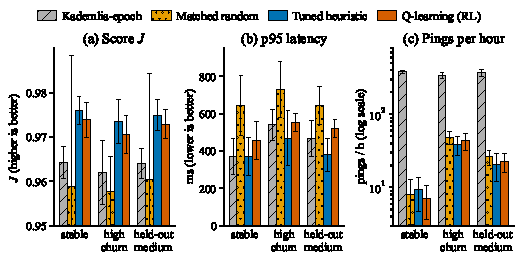
\includegraphics[width=\columnwidth]{fig_results.pdf}
\caption{Mean score $J$, p95 latency and maintenance pings per hour (logarithmic axis) for each scenario; Q-learning is shown in red. Error bars show one standard deviation across the 20 evaluation seeds.}
\label{fig:res}
\end{figure}

\begin{table}[t]
\centering\footnotesize
\caption{Pre-registered hypotheses and final verdicts (source: \texttt{hypotheses.csv}).}
\label{tab:hyp}
\setlength{\tabcolsep}{4pt}
\begin{tabular}{@{}l >{\raggedright\arraybackslash}p{6.3cm} l@{}}
\toprule
ID & Statement & Verdict\\
\midrule
H1 & RL beats matched random on $J$, every scenario (Holm) & pass\\
H2 & high\_churn: RL non-inferior (1\,pp success) to Kademlia-epoch and tuned heuristic, and better on $\ge 1$ of success, p95, pings & inconclusive\\
H3 & Pings $\le$ Kademlia-epoch; p95 $\le 1.05\times$ best baseline (all) & fail\\
H4 & H2 holds on heldout\_medium & inconclusive\\
H5 & All 3 RL runs agree with pooled direction (high\_churn) & pass\\
\bottomrule
\end{tabular}
\end{table}

\section{Exploratory Ablations}
These ablations are \emph{not} part of the primary evaluation. They were run post hoc on separate TEST seeds (disjoint from the evaluation seeds) without multiple-comparison correction; they suggest hypotheses but confirm none.

\inl{Agent ablations} Permuting rewards across an episode's transitions lowers $J$ by about 0.008--0.012 relative to an unshuffled control, and $\gamma=0$ performs worse in all three scenarios. The learned behaviour therefore depends on the reward signal and, to a lesser extent, on multi-step credit assignment. None of the 11 variants reached the tuned heuristic.

\inl{Latency-weight sweep} Retraining with a larger $w_L$, scored under the canonical weights, was associated with lower RL p95 latency (e.g., $-131$\,ms in stable at $w_L=1.0$) but with 74--100 instead of 8--44 pings/h. In high\_churn, RL's p95 remained above the tuned heuristic's. One cell exceeded the tuned heuristic on stable $J$, but it was selected post hoc from 36 combinations and has not been validated. The sweep does not establish that the latency weight explains the gap.

\inl{Memoryless churn} With Weibull shape 1.0, the policy ranking was unchanged, and RL's gap to the tuned heuristic did not shift detectably ($+0.0007$ [$-0.0004$, $+0.0018$]).

\section{Conclusions and Limitations}
\inl{Supported by the primary evaluation} In this simulator, a tabular Q-learner over 540 observable states outperforms Kademlia-style epoch maintenance on $J$ in all three scenarios at far lower maintenance-ping rates, by targeting its decisions rather than merely acting less. \inl{Not supported} RL does not match the tuned 32-configuration heuristic, which achieves higher $J$ and lower p95 latency. We make no claim about real-world deployments.

\inl{Limitations} The study uses a single custom simulator with atomic lookups, perfect storage, 128 nodes and one adapting node. Headroom is small: success without any maintenance is already 98.3--99.5\%, so most of the signal lies in latency and cost. The state is hand-binned and tabular under partial observability; there are only 20 evaluation seeds and 3 training runs; and the tuning budget favours the heuristic (32 configurations versus 4 RL grid points). Kademlia-epoch quantises Kademlia's rule to 30\,s epochs, and bursty churn was not simulated.

\inl{Future work (proposed, not performed)} Simulate and evaluate correlated churn; confirm the exploratory leads on fresh, pre-registered seeds; re-tune the heuristic jointly with the reward weights and compare latency--ping Pareto fronts; and test larger networks and non-atomic lookups. Details: \texttt{FINAL\_RESULTS.md}.


\begin{thebibliography}{9}\footnotesize
\setlength{\itemsep}{1pt}
\bibitem{kad} P.~Maymounkov and D.~Mazi\`eres, ``Kademlia: A peer-to-peer information system based on the XOR metric,'' in \emph{Proc.\ IPTPS}, 2002.
\bibitem{wat} C.~J.~C.~H. Watkins and P.~Dayan, ``Q-learning,'' \emph{Machine Learning}, vol.~8, no.~3--4, pp.~279--292, 1992.
\bibitem{sb} R.~S. Sutton and A.~G. Barto, \emph{Reinforcement Learning: An Introduction}, 2nd ed. MIT Press, 2018.
\bibitem{kaelbling} L.~P. Kaelbling, M.~L. Littman, and A.~R. Cassandra, ``Planning and acting in partially observable stochastic domains,'' \emph{Artificial Intelligence}, vol.~101, no.~1--2, pp.~99--134, 1998.
\bibitem{holm} S.~Holm, ``A simple sequentially rejective multiple test procedure,'' \emph{Scandinavian Journal of Statistics}, vol.~6, no.~2, pp.~65--70, 1979.
\end{thebibliography}

\end{document}
